\chapter{Transformers and the Generative Pre-Training 2 Transformer}
\label{chapter-transformer}

\section{Transformer and Attention}

\label{transformer-intro}

The Transformer is a mechanism that is based entirely on attention. Strictly speaking, this is not the attention explored in the sequence-to-sequence model in Section \ref{section-gru-attention}, though there are some similarities. It is a model that uses no recurrent components.

Recurrent components have some negative qualities. They are hard to run with batch input data. In addition they do not work with very long data strings. 


Transformers use no Recurrent Neural Network components. Their operations can be parallelized so that large batches of data can be processed at once during the same time step. Longer sequences can be considered as well, so Transformer input can contain longer English language sentences and even paragraphs. 

Transformers are usually constructed on eight or more of these layers in the decoder and the encoder. One layer is discussed below.

\subsection{Byte Pair Encoding}

\ac{BPE} stands for ``Byte Pair Encoding.'' WordPiece is a particular implementation of BPE. WordPiece is used by some Transformer systems to encode words much the way that Word2Vec does. Like Word2Vec, WordPiece  has a vocabulary list and a table of embeddings that maps one word, or token, to a vector of a given size.

WordPiece, though, handles Out Of Vocabulary (\ac{OOV}) words gracefully. It breaks large words into smaller pieces that are in the vocabulary, and has a special notation so that these parts can easily be recombined in order to create the input word again. Byte Pair Encoding doesn't use pre-trained word embeddings as do Word2Vec and GloVe.

For the Generative Pre-Training 2 transformer, a version of BPE is used instead of a vocabulary system like Word2Vec or GloVe. Some form of BPE is included in almost every Transformer type Neural Network model, so no decision needs to be made about what type of word embeddings to use.

\subsection{Attention}
Attention mechanisms are used in a similar way in three places in the Transformer model. The first implementation of Self Attention is discussed below. Each of these attention mechanisms is contained in a layer. There are typically the same number of layers in the encoder as in the decoder.

Input to the Transformer is composed of strings of words from a desired input language. Output is composed of words in a given language. Input words are treated very much the way that they are in sequence-to-sequence models. A word is translated to a number and that number indexes an entry in a word-to-vector table. From that time forward, a word is represented by a vector of floating point numbers. In a Transformer this word vector can be large. In the original paper, Vaswani et al \cite{Vaswani2017AttentionIA} use a vector size of 512. The discussion of Generative Pre-Training 2 will see vector sizes of 768 and 1280.

\begin{figure}[H]
	\begin{center}
		
		
		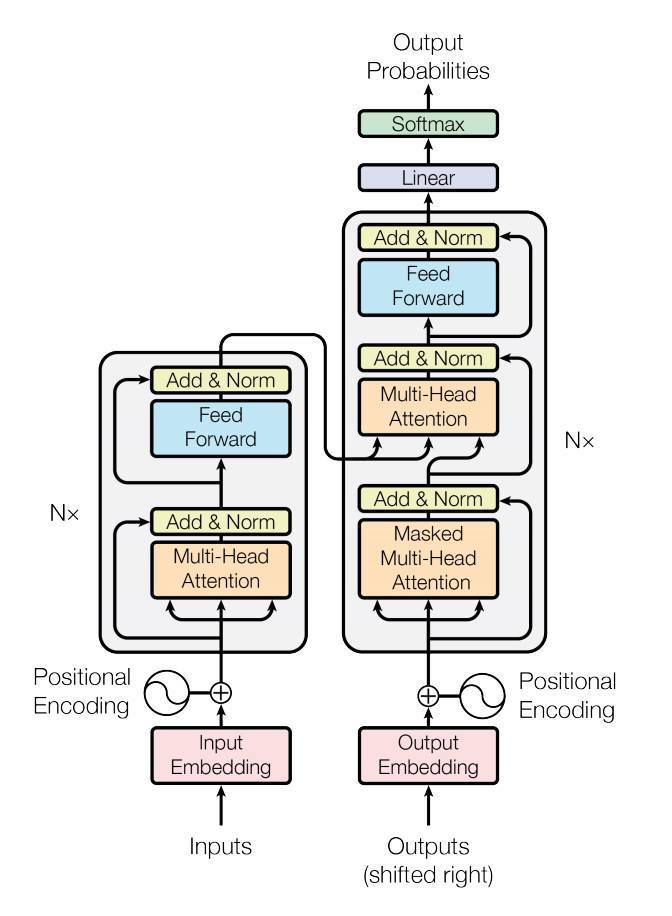
\includegraphics[scale=1.5]{diagram-mat04}
	\end{center}
	\caption[Transformer Encoder and Decoder]{Transformer Encoder and Decoder. - $Nx$ shows number of layers. (Data travels from the bottom to the top.) - Vaswani et al \cite{Vaswani2017AttentionIA}}
	
	
\end{figure}

\subsection{Encoder - Scaled Dot-Product Attention}

Each layer of the Transformer's encoder has a signature self-attention mechanism. This is possibly one third of the entire Transformer mechanism, but a variety shows up in the other two-thirds. 

Initially the input word vectors are converted to three other values. These vectors are similar to the input vector but they have a smaller dimensionality. Converting the word vectors in this way is accomplished by three simple matrix multiplication operations.

Figure \ref{diagram-mat-mult-01} shows a simple conversion of this type. In the diagram a conversion of a vector with dimension of 1x3 to a dimension of 1x2 is shown. In a real world example matrices are converted from a vector of 1x512 to 1x64, a division of 8.



\begin{figure}[H]
	\begin{center}
		
	
	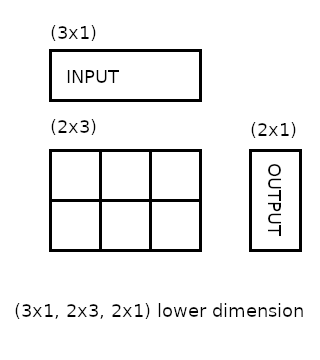
\includegraphics[scale=0.5]{diagram-mat01}
\end{center}
	\caption[Lowering Dimensionality]{Lowering Dimensionality}
	
	\label{diagram-mat-mult-01}
\end{figure}

In the Transformer, this conversion operation is probably the reason for the model's name. The input is \textit{transformed} to a lower dimension. 

The dimension of the starting vector must be preserved. The starting vector is of floating point numbers sized 512. After some processing the vector is converted to smaller 64 sized floating point numbers. The final output of the attention mechanism must be sized 512. %Before that is done the vector is processed at the smaller size of 64 floating point numbers. 

In this self-attention scheme three vectors are actually required. All three vectors are sized 64, and all three are converted by separate matrix multiplication operations. The weights to convert each of the three vectors are different. For this reason the new smaller vectors are all different.

The smaller vectors individually are called q, k, and v. They can also be referred to as larger matrices. The new vector matrices are denoted as Q, K, and V. Q stands for ``Query.'' K stands for ``Key.'' V stands for ``Value.'' The lower-case names refer to single vectors and the upper-case refer to matrices. These are essentially batches of input.

The Query value is multiplied by the Key values from all vectors in the input. This multiplication is ``dot-product'' multiplication. When it is done, all keys will have low output values, except those that are closest to the Query. Then the results are passed through a softmax function. When this is complete, there will be a single vector that is close to 1 and another group of vectors that are all close to 0.

The vector produced by multiplying the softmax with the V values of every word produces a single word vector that is close to its original value, and many others that are near zero. This formula from Vaswani et al \cite{Vaswani2017AttentionIA} shows the process.

$$
\mathlarger{ \mathlarger{
Attention(Q,K,V)=softmax(\dfrac{QK^T}{\sqrt{d_k}})V
} }
$$

The value of $\sqrt{d_k}$ is used to limit the size of the $QK^T$ output. The $d_k$ is the dimension 512. Without this, the softmax function has to deal with much larger numbers. Smaller numbers for the softmax are preferred. $K^T$ is notation for the $K$ vector transposed.

The function can actually perform this on large matrices with high dimensionality, in parallel. This parallel matrix operation increases the speed of training.

In the triangle in the Figure \ref{attantion-7} the multiplication and selection that was just described is performed.

\begin{figure}[H]
	\begin{center}
		
		
		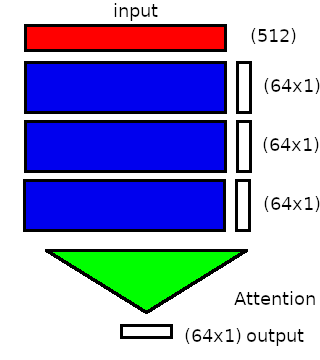
\includegraphics[scale=0.5]{diagram-mat04-64}
	\end{center}
	\caption[Attention Output]{Attention Output. (Data travels from the top to the bottom.)}
	
	\label{attantion-7}
\end{figure}




Finally the output calculated above must be returned somehow to the input dimensionality. This is accomplished by duplicating the procedure described eight times with eight separate weights. When this is done the output of the eight separate attention mechanisms is concatenated together, returning the output to the proper size. This multi-headed approach allows different heads to learn different types of relationships and, then when they are grouped together, the learned relations are recovered and contribute to the output.

\begin{figure}[H]
	\begin{center}
		
	
	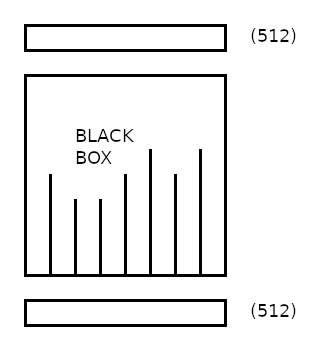
\includegraphics[scale=0.5]{diagram-mat02}
\end{center}
	\caption[Matching Input and Output]{Matching Input and Output. (Data travels from the top to the bottom.)}
	\label{attention-matching}

\end{figure}


Later the output is passed through a feed forward network. It is also combined with the original input again through addition. Then the output is normalized. This ensures that the values are all within reasonable ranges. This recombination of the attention output with the original output is done throughout each Transformer layer.

This describes the encoder section. There are two other attention segments. Together these two sections combine to form the decoder section. This is repeated for each layer.

\begin{figure}[H]
	\begin{center}
		
		
		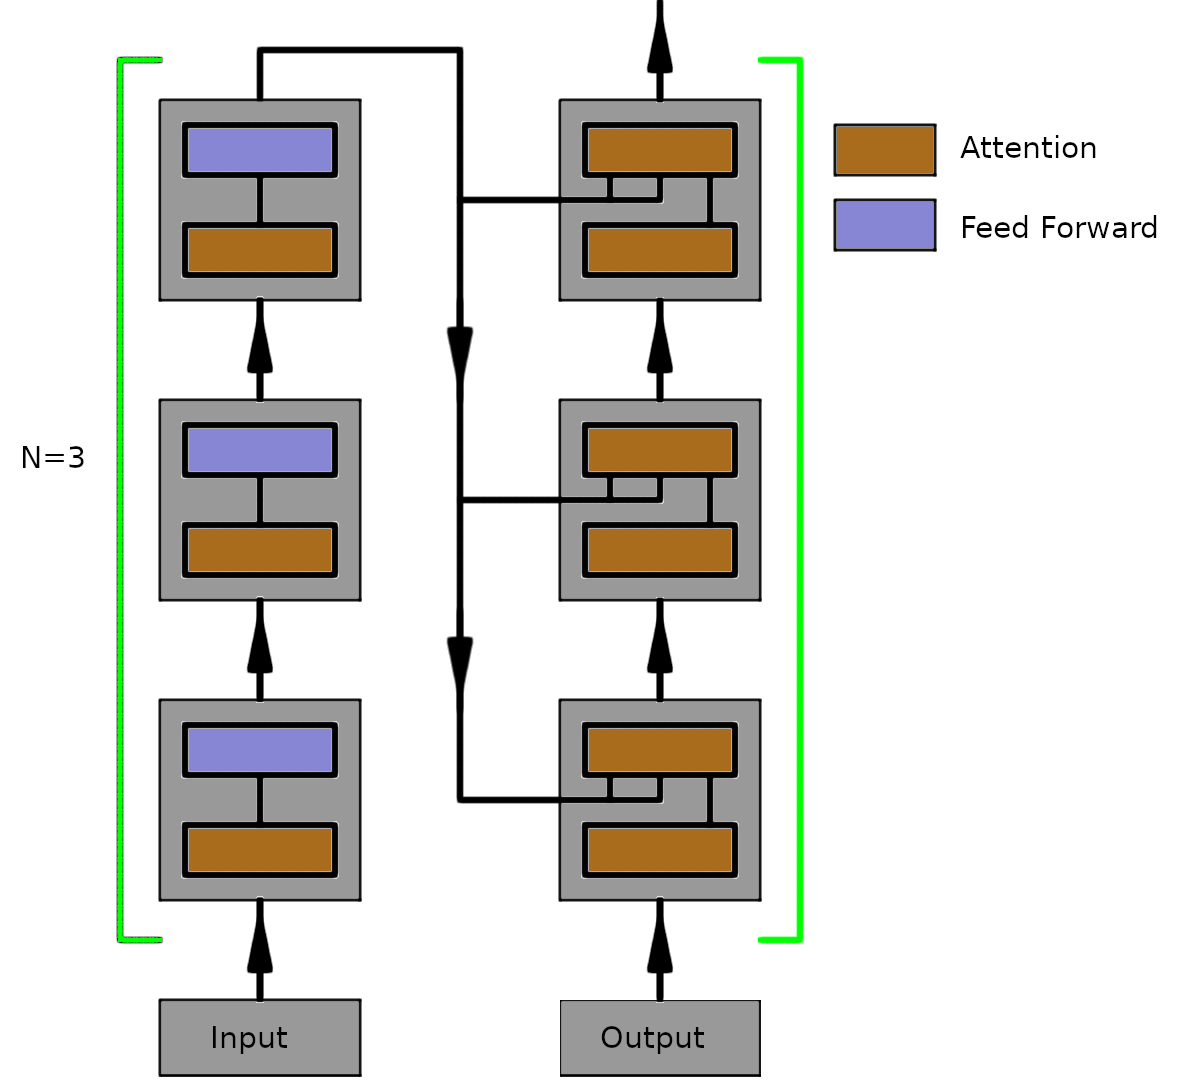
\includegraphics[scale=1.0]{diagram-flow1}
	\end{center}
	\caption[Transformer Encoder and Decoder Flow]{Transformer Encoder and Decoder Flow. - Three layers and data flow. (Data travels from the bottom to the top.)}
	\label{diagram-flow1}
	
\end{figure}

In the flow diagram, Figure \ref{diagram-flow1}, most sub-segments of the entire transformer are not described. The focus is the flow of data through the three encoder segments and the different flow of data through the decoder segments. The encoder is largely serial, while the decoder is serial and parallel. In fact each decoder segment includes a feed forward part, and all decoder and encoder parts include a residual connection where the input is added back to the output of the attention and feed forward segments.

The output of the encoder is a group of vectors the same size as the input sequence. They become the ``Key'' and ``Value'' batches below. The encoder section iterates once for every input data sequence.


\begin{figure}[H]
	\begin{center}
		
		
		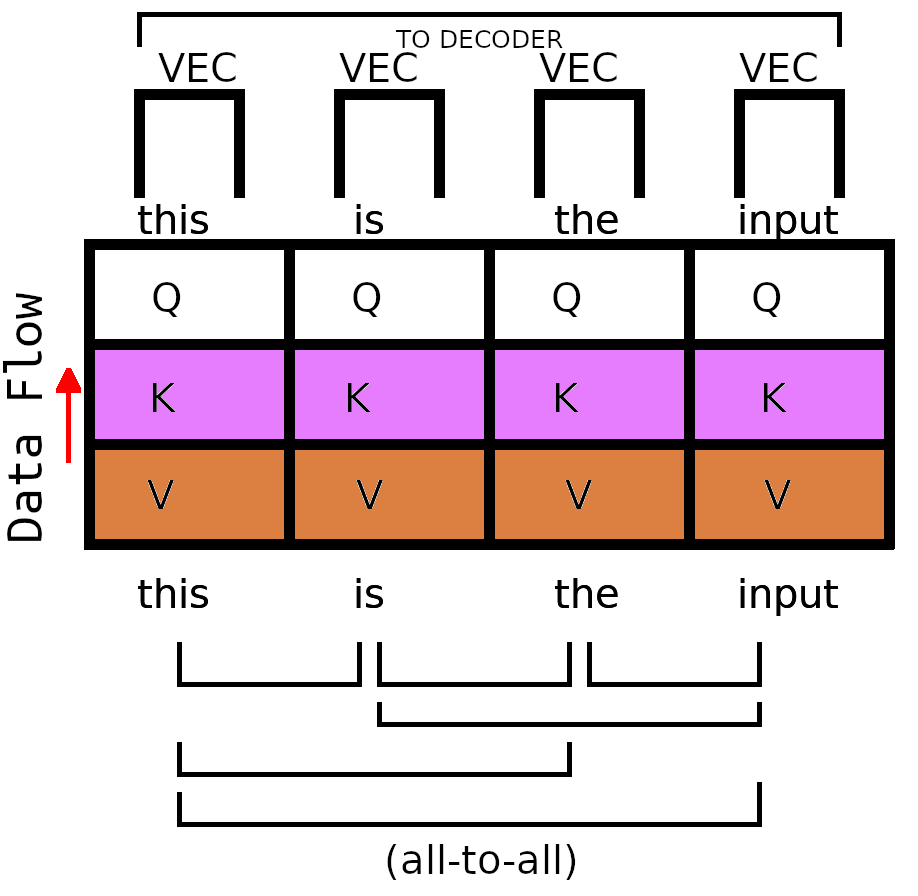
\includegraphics[scale=0.75]{diagram-graph-encoder-flow-b}
	\end{center}
	\caption[Encoder Attention Detail]{Encoder Attention Detail. (Data travels from the bottom to the top.)}
	
	
\end{figure}

\subsection{Decoder Attention I - ``Key'' and ``Value''}
The decoder is composed of two attention mechanisms and a feed forward segment at each layer. The result of the encoder's work is passed to the decoder and remains applied to one of the decoder's attention mechanisms in each decoder layer. In one attention mechanism of the decoder, the ``Key'' and ``Value'' matrices are imported from the encoder. 

While the encoder takes in the entire input and attends to whatever portion of that input it finds to be important, the decoder is interested in producing one output token at a time. The decoder section iterates once for every output word. Throughout this process the information from the encoder does not change. In the flow diagram one layer of the decoder is illustrated.

\begin{figure}[H]
	\begin{center}
		
		
		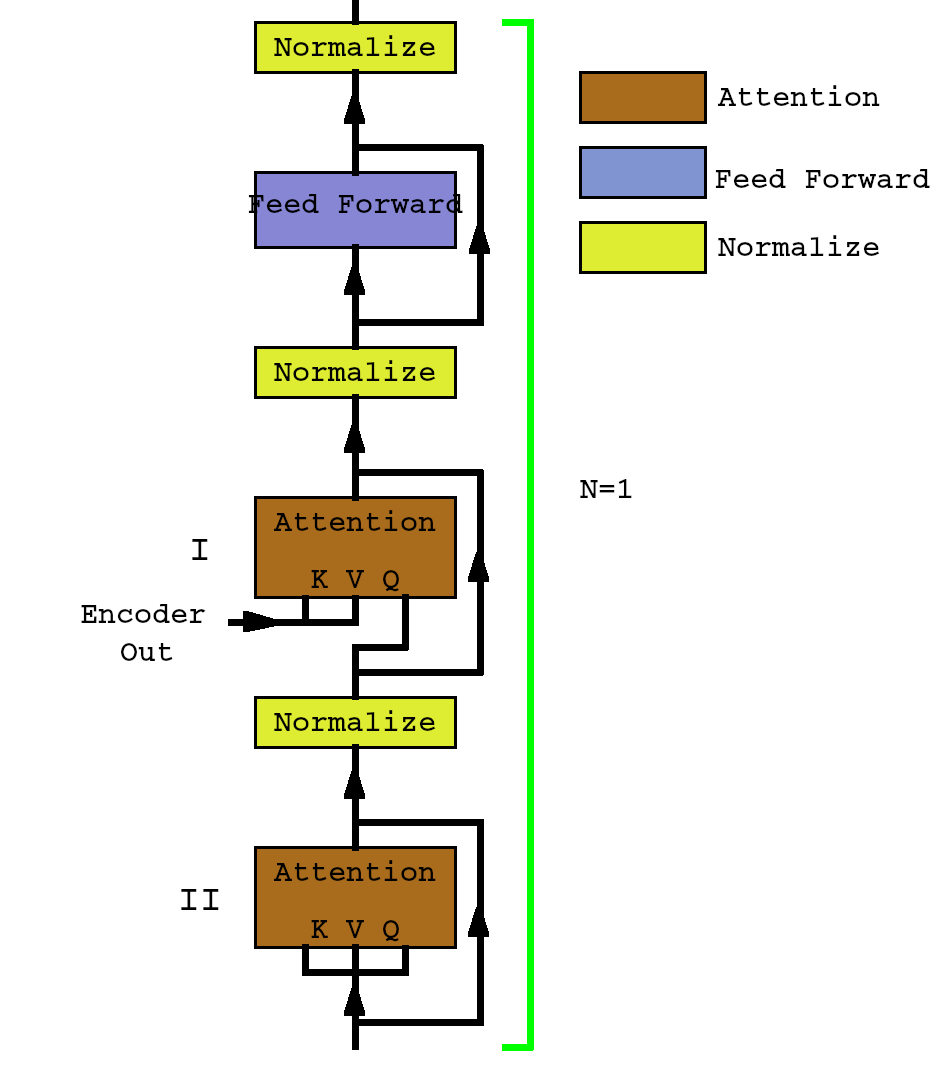
\includegraphics[scale=1.25]{diagram-flow-decoder02}
	\end{center}
	\caption[Decoder Flow]{Decoder Flow Details - ``I'' for encoder-decoder attention. ``II'' for masked decoder self-attention. (Data travels from the bottom to the top.)}
	
	
\end{figure}


Illustrated in the sequence-to-sequence discussion was the importance of the single ``thought vector.'' The Transformer can be seen as having a thought vector also. There is a corridor of data from encoder to decoder. It is composed of a sequence of vectors the size of the input sequence or sentence. It is larger, strictly speaking, than a single vector.

Two important smaller vector-sized inputs from the encoder are ultimately required in all layers of the decoder. They represent the ``Key'' and ``Value'' matrices from the thought vector. The matrices required are the size of the smaller reduced vector. The full sized vectors are transported from the encoder and are reduced dimensionally in the decoder layers to a sequence of two smaller matrices. 

These full sized vectors come from the last encoder layer's output. Typically there will be as many decoder layers as there are encoder layers. The output from the last encoder layer is applied to the ``Key'' and ``Value'' inputs of one of the attention mechanisms in all the decoder layers.
\begin{figure}[H]
	\begin{center}
		
		
		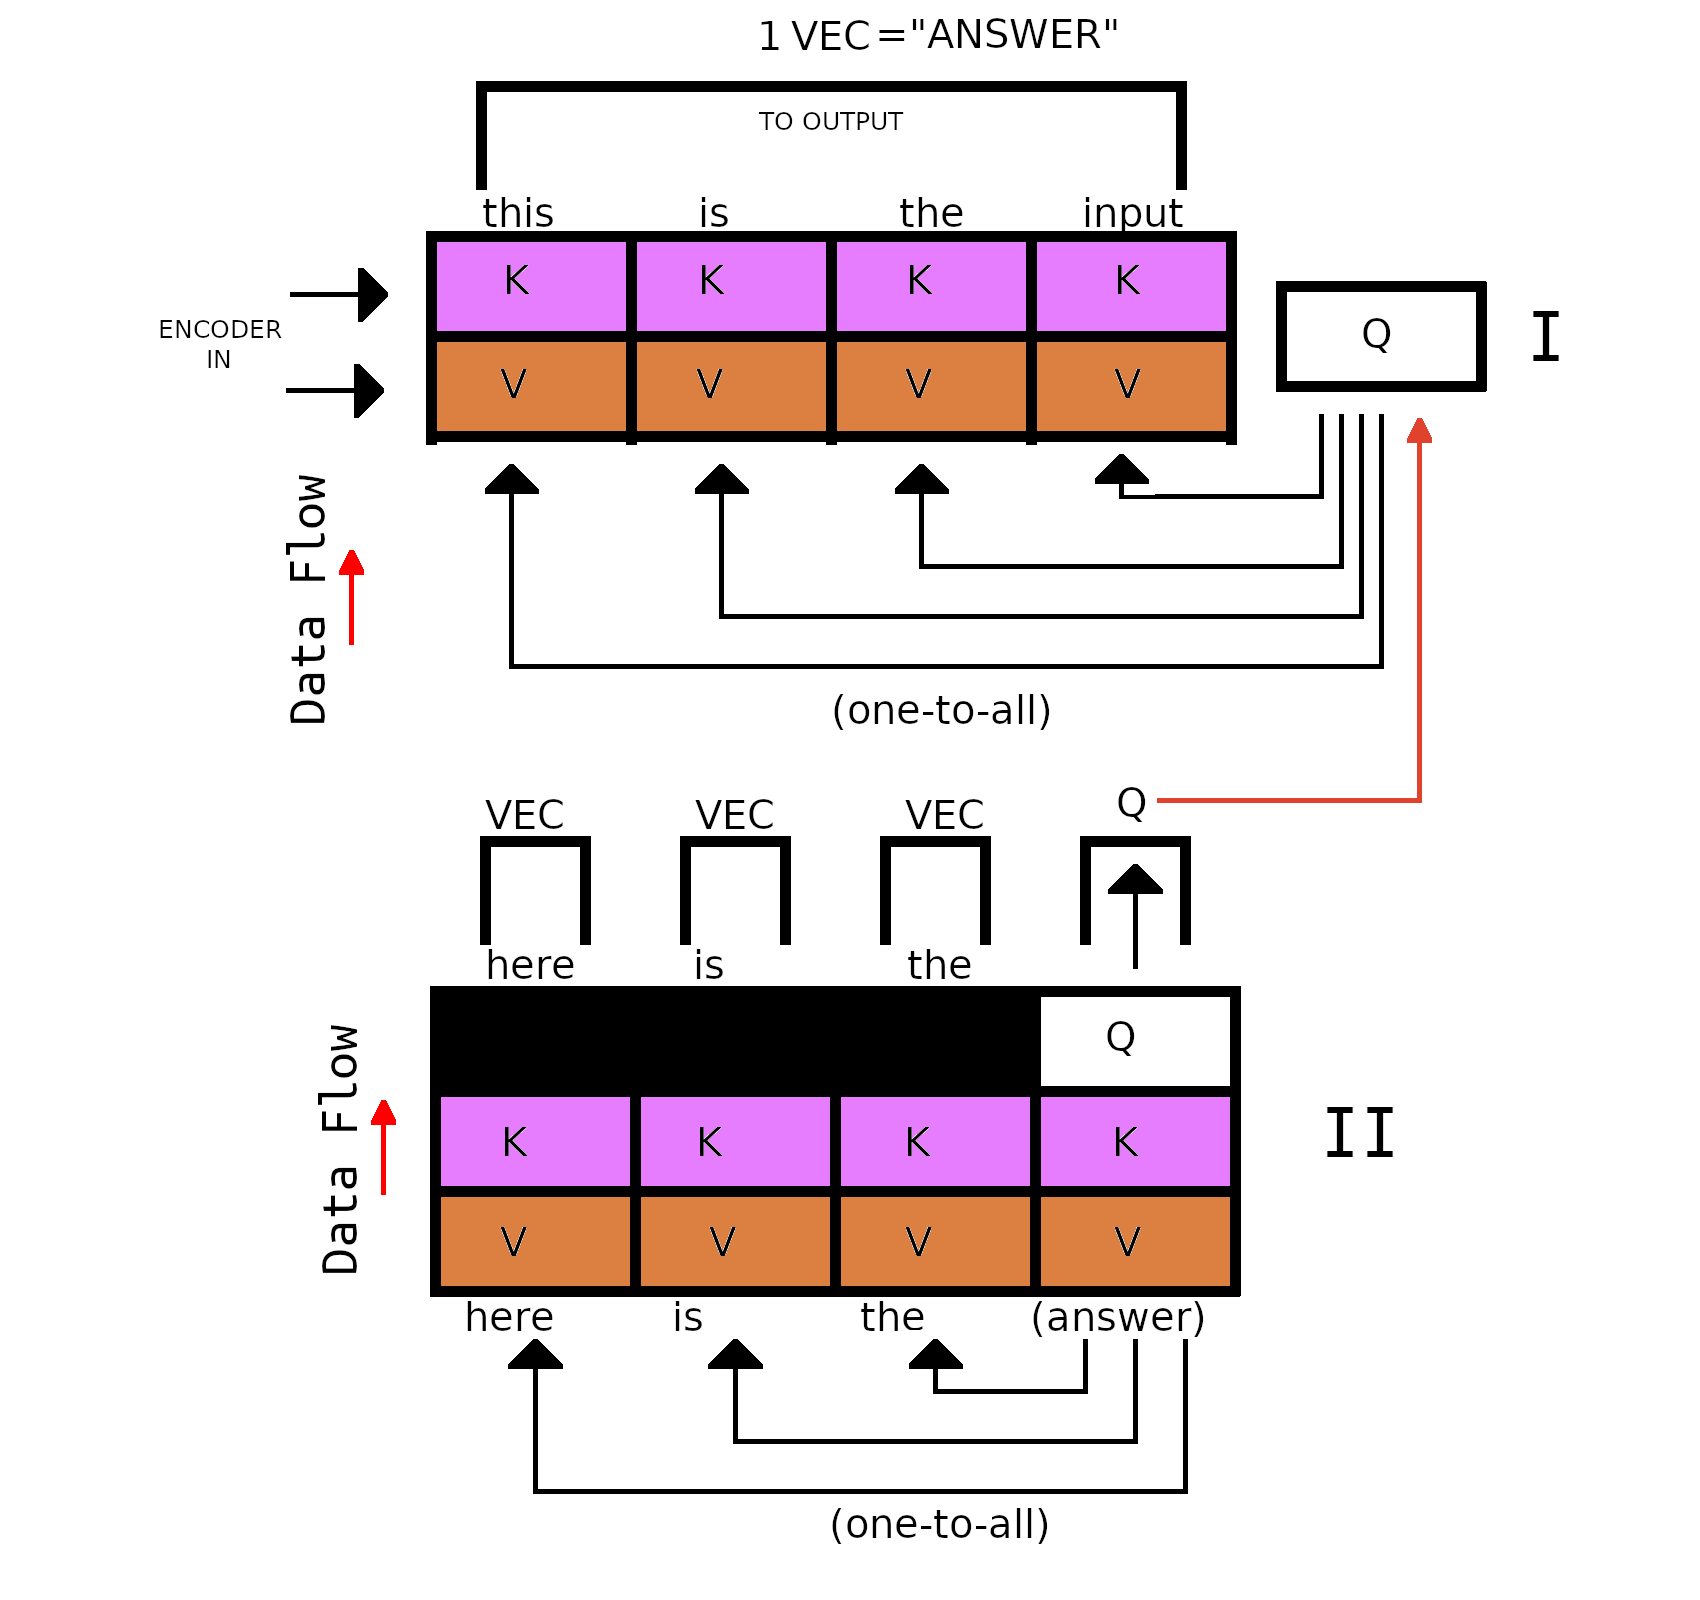
\includegraphics[scale=0.75]{diagram-graph-decoder-flow-c}
	\end{center}
	\caption[Decoder Attention Detail]{Decoder Attention Detail. (Data travels from the bottom to the top.)}
	
	
\end{figure}


\subsection{Decoder Attention II - ``Query''}
There is another attention mechanism in each decoder layer. It works solely on data from the decoder itself. It works very much like the attention mechanism from the encoder, but it attends to every word of output as opposed to the entire input sequence. It passes its output to the attention mechanism described above. This data is lowered in dimensionality and becomes the ``Query'' matrix for that mechanism. 

The ``Key'' and ``Value'' sequences from the encoder are a group of vectors the size of the input sequence. The ``Query'' matrix is the size of a single vector. This is because the decoder is interested in predicting one word at a time. This section produces a single vector as well.


\subsection{Decoder Attention II - Masking}
Input for the second decoder attention section is a group of vectors from the output generated thus far. During inference this output grows by one token with every pass through the decoder. This is how text is generated.

During training the second decoder section is masked. The mask prohibits the decoder from seeing parts of the target. This mimics the inference setup. In inference the decoder can only see up to the most recent word it has produced.

During inference the decoder produces a sentence one token at a time. Then it adds to that sentence, one token at a time, until the decoding is finished and something like English is produced. It can attend to any part of the output it has already produced. It is concerned with producing a single token at a time. These tokens strung together are the output of the Transformer. This output should be readable. 

More information about how this part of the decoder works can be found in Section  \ref{pre-trining-2-model}. Attention in this part of the Transformer is very similar to the GPT2.

\begin{figure}[H]
	\begin{center}
		
		
		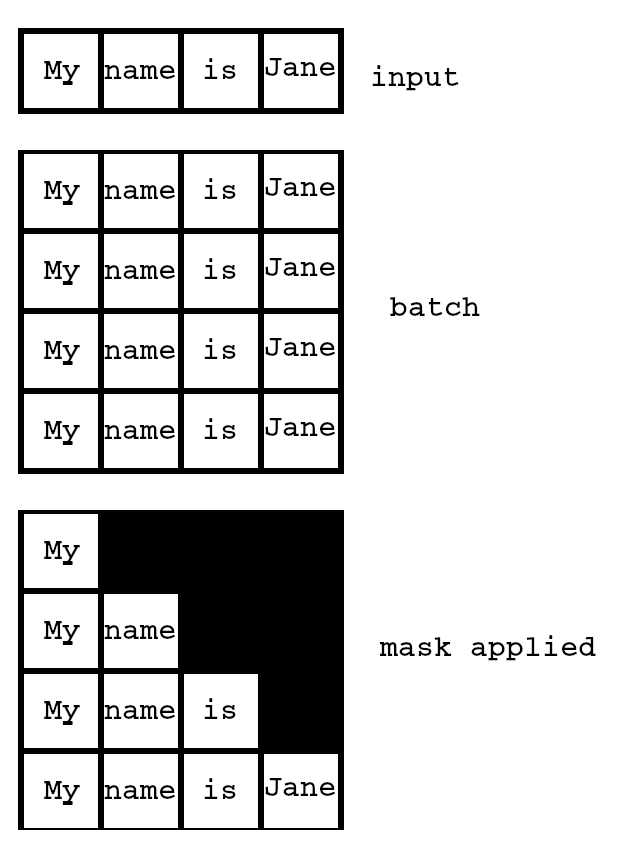
\includegraphics[scale=1.25]{diagram-mask01}
	\end{center}
	\caption[Decoder Mask]{Mask. - Decoder uses masked input during training.}
	
	\label{diagram-mask-01}
\end{figure}



%\subsection{Transformer - General}
\subsection{Input - Positional Encoding}
The input of the Transformer encoder and decoder layers employ not only a word vector table, but also a positional encoding scheme. The model adds sine and cosine patterns to the input vector that it can then use to learn the position of words in a sentence. 

Words that are early in the sentence have a certain appearance and words later on appear differently. The encoder and decoder use the sine and cosine waves to impart this information onto the sentence sequence. 

\subsection{Output - Feed Forward Network}
At the output of the last layer of the decoder, the output vectors are processed through a linear matrix which increases the vector's dimensionality, so that the output vector is the size as the output vocabulary dimensionality. After the linear matrix the vector is processed by a softmax function. Then the highest floating point value in the new larger vector is the index of the chosen output word.


\subsection{Visualization - Transformer}

A colorful chart is used to visualize what is happening during inference. This chart illustrates how each word attends to all the other words in the input text.

\begin{figure}[H]
	\begin{center}
		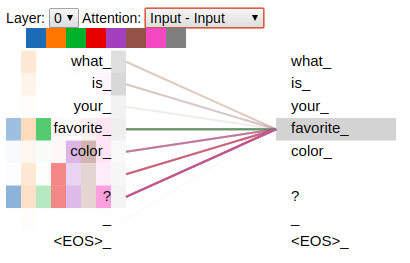
\includegraphics[scale=2]{Figure_3}
		
		
	\end{center}
	\caption[Visualized Attention Transformer]{Visualized Attention -- ``favorite'' shows attention to some but not all words in the sentence.}
	
	
\end{figure}

It is significant that words like ``what'' and ``your'' do not have strong attention to other words in the text. In a chart like this one they would show no colors on the left and light colored lines connecting the right to the left. This diagram is from the Transformer with the larger hyper-parameter set that is described in Chapter \ref{chapter-approach-to-study}, trained on the movie dialog corpus.


\section{The Generative Pre-Training 2 Model}

\label{pre-trining-2-model}

``Generative Pre-Training 2'' is a large model. It is based on the Transformer from Vaswani et al \cite{Vaswani2017AttentionIA} but there are some major changes. The model uses the decoder portion of the Transformer without the encoder. There are other changes to the output layers. Furthermore it is pre-trained and downloadable. The GPT2 model is used to create some of our chatbots.


\subsection{Pre-Training}
In Pre-Training the authors of a model train an instance and then make the model available to the user on-line. This is helpful for the average programmer interested in Neural Networks. Training an instance of the Transformer model can use computational resources for days, and require hardware that is costly. Usually the cost of producing a trained model is prohibitively expensive.

After acquiring a trained model, programmers go on to adjust the model to their task. Adjusting a pre-trained model to a given task is called ``Transfer Learning.'' Many tasks lend themselves to Transfer Learning. Conceptually a model can be fine-tuned to many problems. % and many problems can be addressed with good results after only modest fine-tuning.


\subsection{General}
\ac{GPT2} still uses Scaled Dot-Product Attention. A model diagram is taken from Radford et al \cite{radford2018improving}. 

\begin{figure}[H]
	\begin{center}
		
		
		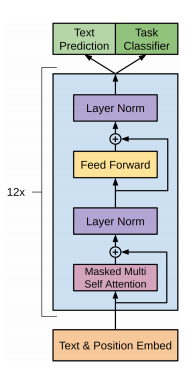
\includegraphics[scale=3.0]{diagram-mat05}
	\end{center}
	\caption[Generative Pre-Training 2 ]{GPT2 - Radford et al \cite{radford2018improving}. (Data travels from the bottom to the top.)}
	

\end{figure}

There are several sizes of pre-trained GPT2 models, all rather large. The smallest model has 12 layers, while the Transformer model in the example from Vaswani et al \cite{Vaswani2017AttentionIA} uses 8 layers. This model also has a hidden dimension of 768, not 512. With 8 heads this leaves a smaller dimensionality of 96 at each attention head. 

%The GPT2 models input and output text sequences.


\subsection{Training}

The GPT2 model is trained on text from the web, specifically Reddit. The goal for training is to show the model part of a large piece of text and then to have the model predict the next word. A mask is used in the Self Attention segment of the model during training.

%For this task the mask is important. Training could consist of incrementally showing a model text at different states of completion and then asking it to predict the next token. In this kind of arrangement the batch sizes would be shorter and focus on each word. 

Training could present the model with the text in complete form and have the model look at it through a mask. A mask is visualized in Diagram \ref{diagram-mask-01}.

Each word would have an opportunity to be focused on as the ``next'' word. A boundary is formed between the last word and the masked area to its right. The boundary between each word and the one that follows it is examined. The model can still be trained on large batches in parallel. Words to the right of the last word and the particular boundary being examined are not available to the model.

Training is done by the developers of the model and the authors of the paper. The model is too big for individuals to train from scratch. 

\subsection{Inference}

In this example creating ``conditional samples'' are discussed, in contrast to creating ``unconditional samples.'' Conditional samples rely on an input sequence for generating output. Unconditional samples have no input specified. %A mask is not used during inference.

First a series of input tokens must be selected for the example. This series of tokens is generated from an English sentence. The sequence used will be ``Good day'' for this example. The words in the sequence translate into single tokens in the corpus. An input word may be made up of several tokens, but that should not be the case in this simple example.

The input context for GPT2 models is 1024 tokens. Here the input tokens, ``good'' and ``day,''  take up two spots in the input area. They are followed by an end-of-sequence token. Together they take up three spots. At that time there are 1021 spots left in the input area.

The first words are converted to tokens and are passed through the embedding matrix where they are converted to vectors. Positional encoding patterns are generated for each of the three vectors. These positional encoding patterns are created from sine and cosine waves that are concatenated together. They are added to the input tokens.

The model starts at the fourth location and attempts to generate the next token. The entire model is at this moment addressing the task of generating the next token.

One of the important processes that the input goes through is the Scaled Dot-Product Attention. This is performed at each layer. There are 12 layers in the 117M model.

All three tokens are converted to smaller vectors for each layer. Then the third vector, for the end-of-sequence token, is treated as the ``Query.'' The matrices for the ``Key'' and ``Value'' are assembled from the words in the input. This is done for all of the heads of each individual layer.

At this time, the model is making the transition from the third spot to the fourth spot.

The third word ``Query'' vector, the end-of-sequence, is compared to each other previous word ``Key'' vectors using dot-product multiplication. Then the result is Softmaxed, producing a single vector that is close to 1 and a group of all other vectors that are closer to 0. The result of that is multiplied by all of the three ``Value'' vectors. A single result is found in this way.

The output is concatenated together at each layer across all the heads at that layer. The output is recombined with the input. There are also components in each layer that do normalization. Ultimately an output vector is produced that represents what the next token should be. %This vector is converted into a size equivalent to the size of the vocabulary. Then the model can use a method to choose a word from the vocabulary. 

%Frequently, the model looks to the largest floating point number and its association with a word in the vocabulary.

The new token is placed in position four. The first three tokens are left as they are and GPT2 goes back to the start and now looks at the first four tokens as input. It will try to generate the fifth token.

The model will continue to try to generate tokens until the input area is filled and there are 1024 tokens, or a special ``end-of-sequence'' token is generated. The output could be anywhere from 1 to 1021 tokens. This is because the input area starts with a dimension of 1024, and there are three tokens in the original input sentence.


\begin{figure}[H]
	\begin{center}
		
		
		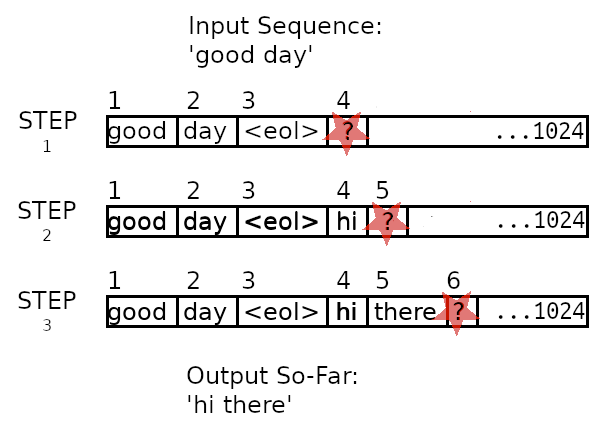
\includegraphics[scale=2.0]{diagram-inference-02}
	\end{center}
	\caption[Generative Pre-Training 2 Inference]{GPT2 - Inference Progress}
	
	
\end{figure}

\subsection{Corpus}
The GPT2 models are trained on a corpus called WebText, a 40GB corpus taken from the Reddit web site. All the material comes from before 2017 and all has a ``karma'' rating of three or better. ``Karma'' is a rating system used internally on Reddit. 

%As with the decoder layer of the Transformer model, the GPT2 model concerns itself with generating words that are later strung together to make sentences or paragraphs. During training the model uses a masking scheme so that input can be parallel-ized. During inference output cannot be parallel-ized, so during inference output must focus on one example at a time.

\subsection{Releases}
In their paper, Radford et al \cite{radford2019language} showed that their model could generate text from a seed sentence or paragraph. At that time the case was made that the largest ``Generative Pre-Training 2'' model should not be released because of its ability to generate text that might fool humans into believing that another person was responsible for the text. Later the larger model was released to the public.

\begin{center}

\begin{tabular}{lrll}
	Size & Parameters & Layers & $d_{model}$ \\
	\hline
	small & 117M       & 12     & 768          \\
	medium & 355M       & 24     & 1024         \\
	large & 774M       & 36     & 1280         \\
	x-large & 1.5B     & 48     & 1600 \\
	xx-large & 8.3B   &  72 &   3072 
\end{tabular}

	
\end{center}
\addcontentsline{lot}{section}{GPT2 Size Overview}

When the first ``Generative Pre-Training 2'' models were released there were three of them. Later two more were trained. The final xx-large model was trained by NVIDIA Applied Deep Learning Research \cite{2019NVIDIAadlr} and was not released to the public.

The ``Generative Pre-Training 2'' models also work in many circumstances in ``zero-shot'' mode, with no extra training to make the model suit the task. It is used ``as is.''

For the chatbot the model using 117 million parameters was successful. Some programming was required to make the model output look like chatbot output, but the model itself was not modified.

Tests were done on both the small and large models. When the larger 774M model was released it was used as a substitution for the 117M model. The test worked, and returned answers that were more well formed than the small model. The larger model does not fit on a Raspberry Pi and so it was not employed here on a permanent basis. %Using the extra large 1.5B parameter model in a chatbot was not attempted at first.

\subsection{Application Details}
The 774M model is described in Radford et al \cite{radford2019language} and the accompanying blog post. The model is trained on English without a stated problem, however large neural network models are usually trained for a stated problem. Rather famously this model is used after training to generate English language text. The model takes input from the user, a premise or summary of what is to be generated. The model also takes as input a number called the ``temperature.'' Then the model generates output. As the ``temperature'' is set higher, the output is more fanciful. There is also a tune-able parameter for the output length. 

%Given the ability of the model to invent content, it was determined by the authors that the `large' model should not be released to the public at first. Months later the `large' model was released. 

For the chatbot the temperature is set to a low number. The length of the output is set to a sentence-length number of tokens. Then as input the output from the speech-to-text translator is used.

The output is not immediately useful. Traditional programming and string manipulation are employed to clean the output and render a short single sentence. %This is the output.

Because the input is meant to be a number of sentences and, because the architecture is Transformer-based, more information can be added to the input string. In this respect the model acts to summarize the input. 

A set of three or four sentences is included with every input string. They suggest the time, the bot's name, and the bot location and occupation. The chatbot summarizes the input. If the information is relevant then it is used by the model as output. %Making this possible is the fact that a Transformer can accept much longer input strings than a Gated Recurrent Unit, and generate much longer output strings.

Surprisingly the chatbot answers most of the questions in the first person. It is felt that WebText, the Reddit corpus, has many examples of sentences in the first person.

\subsection{Visualization - GPT2}

During inference the Scaled Dot Product Attention in the GPT2 focuses on certain words as it processes input text. Here, the word ``favorite'' shows a relationship to many of the other words in the text.  

\begin{figure}[H]
	\begin{center}
		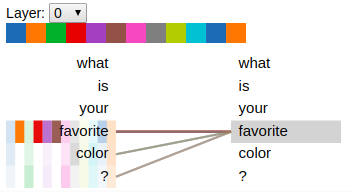
\includegraphics[scale=2]{Figure_4}
		
		
	\end{center}
	\caption[Visualized Attention GPT2]{Visualized Attention GPT2 -- ``favorite'' shows attention to some but not all words in the sentence.}
	\label{diagram-vis04}
	
\end{figure}

The phrase ``What is your favorite color?'' is often answered with ``I love the colors of the rainbow.'' This answer does not mention a specific color, as one might expect it should. Figure \ref{diagram-vis04} might support this observation because ``color'' on the left is not heavily highlighted. Words like ``what'' and ``your'' are barely considered at this head at all. 

